% Provenance (never printed): cycle 4 SVT, "La planete Terre": the dynamics of
% the Earth's outer shell, plates and their boundaries, continental drift as a
% history of ideas; see sources/outline_sources.md. Pilot chapter, 2026-10-22.
\chapter{प्लेट विवर्तनिकी: चलती हुई पहेली}\label{ch:g7:plate-tectonics}

दुनिया का एक \omterm{def:g2:drawing-to-map:map}{मानचित्र} मेज़ पर फैलाओ और अटलांटिक \omterm{def:g2:water-on-earth:ocean}{महासागर} के दोनों किनारों को
देखो। ब्राज़ील का बड़ा उभार ऐसा लगता है मानो अफ़्रीका के पश्चिमी \omterm{def:g1:landscapes-around-us:water}{तट} के खोखले
हिस्से में सरकने के लिए ही बना हो, जैसे किसी ने ज़मीन के एक ही टुकड़े को दो
हिस्सों में काटकर उन्हें एक-दूसरे से दूर धकेल दिया हो। दोनों तटों के अच्छे
\omterm{def:g2:drawing-to-map:map}{मानचित्र} छापने वाले पहले लोगों ने यह तुरंत देख लिया। तीन सदियों तक यह एक
कौतूहल ही बना रहा। बीसवीं सदी में यह उस सिद्धांत का आरंभ-बिंदु बना जो आज
समझाता है कि जापान में ज़मीन क्यों काँपती है, एंडीज़ इतने ऊँचे क्यों हैं,
आइसलैंड धीरे-धीरे चौड़ा क्यों हो रहा है --- और मेज़ पर रखा \omterm{def:g2:drawing-to-map:map}{मानचित्र} एक चलती
हुई दुनिया की बस एक तस्वीर क्यों है।

\begin{omfigure}
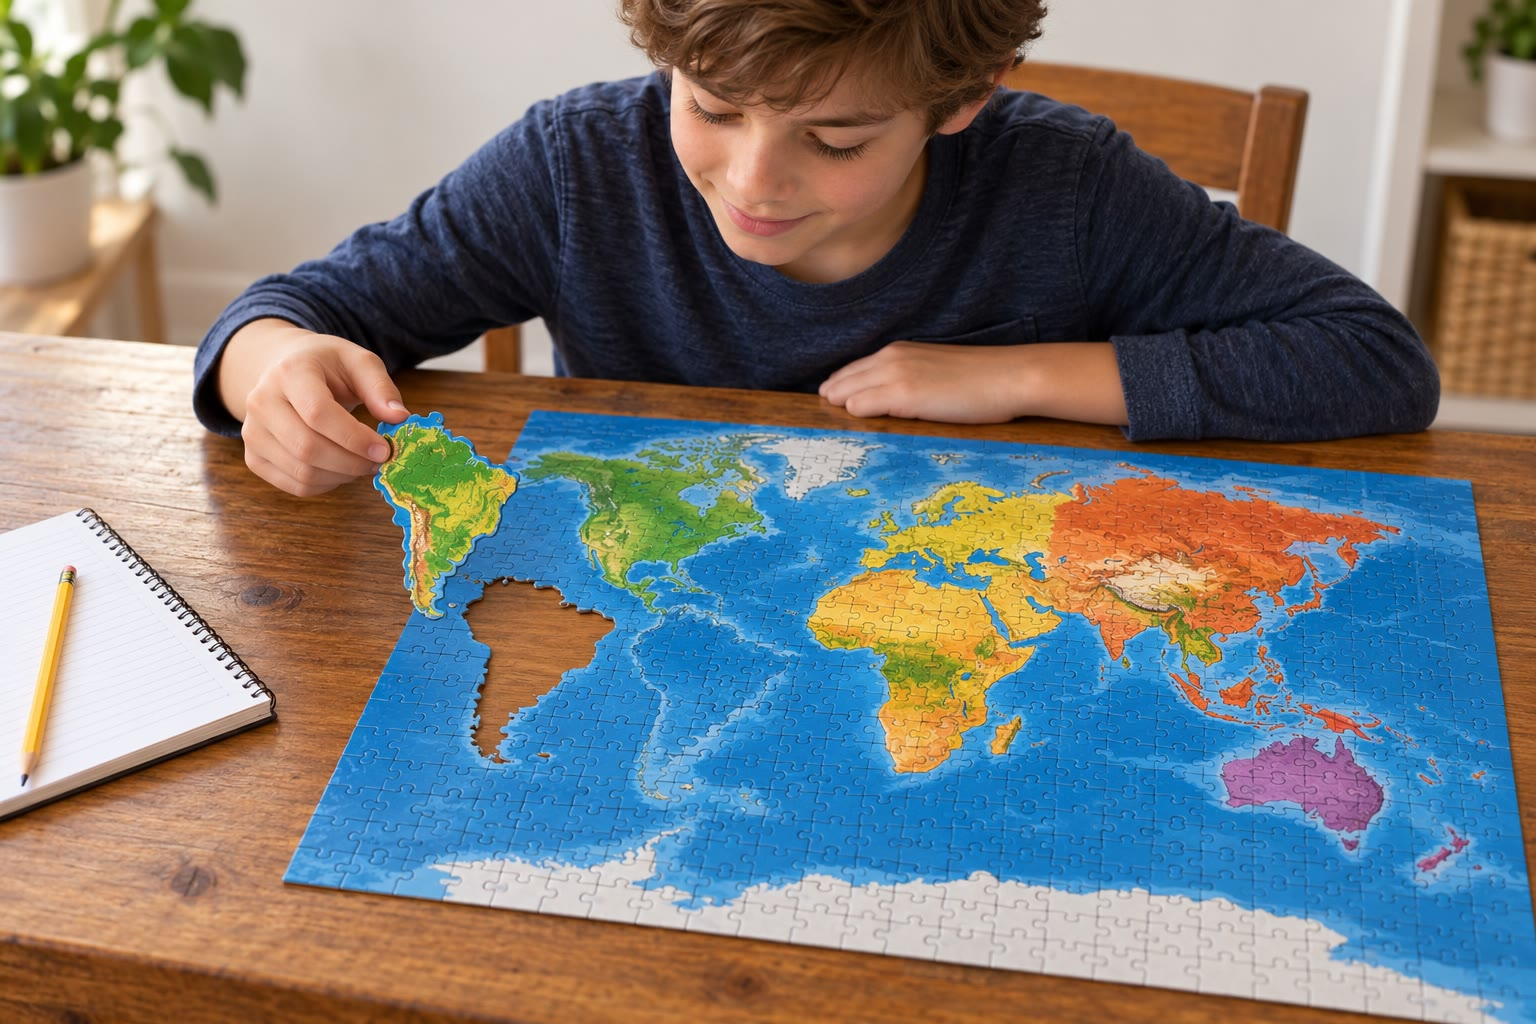
\includegraphics[width=0.62\linewidth]{images/book1/ai/g7-puzzle-map.jpg}

{\small अफ़्रीका के बगल में दक्षिण अमेरिका: एक पहेली में यह मेल एक खेल है;
असली पृथ्वी पर यह एक सुराग है।}
\end{omfigure}

\begin{recall}
पृथ्वी की तीन मुख्य परतें हैं: एक पतली, चट्टानी \emph{\omterm{def:g6:inside-the-earth:layers}{भूपर्पटी}}, गरम \omterm{def:g3:stones-pebbles-sand:rock}{चट्टान}
का एक मोटा \emph{\omterm{def:g6:inside-the-earth:layers}{प्रावार}}, और धातु का एक \emph{\omterm{def:g6:inside-the-earth:layers}{क्रोड}}; गहराई के साथ तापमान
बढ़ता है (\cref{ch:g6:inside-the-earth})। \omterm{def:g3:continents-and-oceans:globe}{ग्लोब} पर किसी जगह की स्थिति उसके
\omterm{def:g6:latitude-longitude:latitude}{अक्षांश} और \omterm{def:g6:latitude-longitude:longitude}{देशांतर} से बताई जाती है (\cref{ch:g6:latitude-longitude})।
\end{recall}

\section{महाद्वीप जो कभी आपस में जुड़े थे}

\begin{definition}[महाद्वीपीय विस्थापन]\label{def:g7:plate-tectonics:continental-drift}
\emph{महाद्वीपीय विस्थापन}\index{महाद्वीपीय विस्थापन} यह विचार है कि
\omterm{def:g3:continents-and-oceans:continent}{महाद्वीप} पृथ्वी की सतह पर धीरे-धीरे चलते हैं, जिससे उनकी स्थितियाँ, और उनके
बीच के \omterm{def:g2:water-on-earth:ocean}{महासागरों} के आकार, युगों के दौरान बदलते
रहे हैं।
\end{definition}

\begin{definition}[महामहाद्वीप]\label{def:g7:plate-tectonics:supercontinent}
\emph{महामहाद्वीप}\index{महामहाद्वीप} ज़मीन का एक अकेला विशाल भूखंड है जो
सभी, या लगभग सभी, \omterm{def:g3:continents-and-oceans:continent}{महाद्वीपों} के आपस में जुड़ने से बना हो। आख़िरी
महामहाद्वीप, \emph{पैंजिया}\index{पैंजिया} (यूनानी में ``सारी ज़मीनें''),
लगभग 225 से 200 मिलियन वर्ष पहले के बीच टूटना शुरू हुआ।
% ledger: usgs:pangaea-breakup
\end{definition}

जिस वैज्ञानिक ने \omterm{def:g7:plate-tectonics:continental-drift}{महाद्वीपीय विस्थापन} का बचाव एक असली सिद्धांत के रूप में,
प्रमाणों के साथ, किया, वे अल्फ़्रेड वेगनर थे। उन्होंने चार तरह के सुराग जुटाए।

\begin{enumerate}
  \item \textbf{तटों के आकार।} दक्षिण अमेरिका और अफ़्रीका एक जिगसॉ पहेली के दो
        टुकड़ों की तरह आपस में बैठ जाते हैं, और कई दूसरी तटरेखाएँ
        भी।
  \item \textbf{जीवाश्म।} एक ही जीवाश्म जानवर और पौधे उन \omterm{def:g3:continents-and-oceans:continent}{महाद्वीपों} पर मिलते
        हैं जिन्हें आज हज़ारों किलोमीटर \omterm{def:g2:water-on-earth:ocean}{महासागर} अलग करता है। \emph{मीसोसॉरस}
        \omterm{def:g2:water-on-earth:salt-fresh}{मीठे पानी} में रहने वाला एक छोटा सरीसृप था: वह तैरकर \omterm{def:g2:water-on-earth:ocean}{महासागर} पार नहीं कर
        सकता था, फिर भी उसके जीवाश्म ब्राज़ील और दक्षिणी अफ़्रीका दोनों में
        मिलते हैं।
  \item \textbf{\omterm{def:g3:stones-pebbles-sand:rock}{चट्टानें}।} एक ही तरह और एक ही उम्र की \omterm{def:g3:stones-pebbles-sand:rock}{चट्टानें}, और एक ही
        आकार की पुरानी \omterm{def:g4:world-physical-map:range}{पर्वत-श्रेणियाँ}, एक \omterm{def:g1:landscapes-around-us:water}{तट} पर रुकती हैं और सामने वाले \omterm{def:g1:landscapes-around-us:water}{तट} पर
        फिर शुरू होती हैं, जैसे फटे हुए अख़बार पर छपी पंक्तियाँ।
  \item \textbf{प्राचीन \omterm{def:g5:weather-and-climate:climate}{जलवायु}।} कोयला, जो गरम, दलदली जंगलों के पौधों से बनता
        है, अंटार्कटिका में मिलता है; प्राचीन हिमनदों के छोड़े निशान अफ़्रीका के
        उन हिस्सों में मिलते हैं जो आज गरम और शुष्क हैं। ये ज़मीनें कभी दूसरी
        \omterm{def:g5:weather-and-climate:climate}{जलवायु} में, दूसरे \omterm{def:g6:latitude-longitude:latitude}{अक्षांशों} पर रही
        होंगी।
\end{enumerate}
% ledger: usgs:coal-antarctica, usgs:fossil-map

\begin{omfigure}
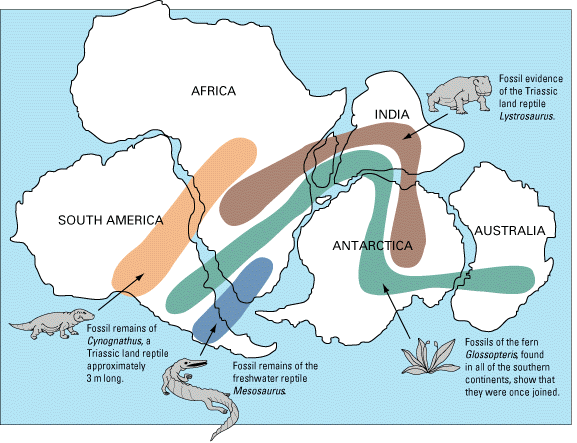
\includegraphics[width=0.86\linewidth]{images/book1/g7-usgs-fossil-map.png}

{\small दक्षिणी \omterm{def:g3:continents-and-oceans:continent}{महाद्वीप} फिर से जोड़े गए। हर रंगीन पट्टी उन जगहों को जोड़ती है
जहाँ आज एक जीवाश्म जाति मिलती है: ज़मीन पर रहने वाले सरीसृप
\emph{साइनोग्नैथस} और \emph{लिस्ट्रोसॉरस}, \omterm{def:g2:water-on-earth:salt-fresh}{मीठे पानी} का सरीसृप
\emph{मीसोसॉरस} और फ़र्न \emph{ग्लोसॉप्टेरिस}। अलग होने पर \omterm{def:g3:continents-and-oceans:continent}{महाद्वीप} पट्टियों
को बिखेर देते हैं; जुड़ने पर पट्टियाँ बिना टूटे आगे चलती हैं। \omterm{def:g2:drawing-to-map:map}{मानचित्र}:
अमेरिकी भूवैज्ञानिक सर्वेक्षण, \emph{दिस डायनैमिक अर्थ} (सार्वजनिक डोमेन)।}
\end{omfigure}

\begin{history}[वेगनर का विचार, 1912--1930]
% ledger: usgs:wegener-1912, usgs:wegener-death, usgs:jeffreys
32 साल के जर्मन मौसम वैज्ञानिक अल्फ़्रेड वेगनर ने 1912 में दो लेखों में
\omterm{def:g7:plate-tectonics:continental-drift}{महाद्वीपीय विस्थापन} का सिद्धांत रखा। ज़्यादातर भूवैज्ञानिकों ने उसे ठुकरा दिया।
सबसे बड़ी आपत्ति यह थी कि वेगनर यह नहीं बता सकते थे कि \omterm{def:g3:continents-and-oceans:continent}{महाद्वीपों} को
\emph{क्या} चलाता है: उनका मानना था कि \omterm{def:g3:continents-and-oceans:continent}{महाद्वीप} \omterm{def:g2:water-on-earth:ocean}{समुद्र} की तली की \omterm{def:g3:stones-pebbles-sand:rock}{चट्टान} को
चीरते हुए आगे बढ़ते हैं, और भौतिकविद हैरल्ड जेफ़्रीज़ ने दिखाया कि ठोस \omterm{def:g3:continents-and-oceans:continent}{महाद्वीप}
टूटे बिना ऐसा नहीं कर सकते। वेगनर प्रमाण जुटाते रहे, जब तक 1930 में एक अभियान
के दौरान ग्रीनलैंड की हिम-चादर पर उनकी मृत्यु नहीं हो गई। जिस जवाब की उन्हें
कमी थी, वह 1950 के दशक के बाद खोजी गई \omterm{def:g2:water-on-earth:ocean}{महासागरों} की तली से आया: उसकी कहानी
बाद के एक वर्ष में सुनाई जाएगी।
\end{history}

\section{प्लेटें}

वेगनर के सुराग सही थे, पर उनके \omterm{def:g3:continents-and-oceans:continent}{महाद्वीप} ग़लत टुकड़े थे। केवल \omterm{def:g3:continents-and-oceans:continent}{महाद्वीप} ही नहीं
चलते: पृथ्वी का पूरा बाहरी कवच, \omterm{def:g3:continents-and-oceans:continent}{महाद्वीपों} के नीचे और \omterm{def:g2:water-on-earth:ocean}{महासागरों} के नीचे एक
जैसा, टुकड़ों में टूटा हुआ है।

\begin{definition}[विवर्तनिक प्लेट]\label{def:g7:plate-tectonics:plate}
\emph{विवर्तनिक प्लेट}\index{विवर्तनिक प्लेट} (या केवल प्लेट) \omterm{def:g3:stones-pebbles-sand:rock}{चट्टान} की एक
बड़ी, कठोर पट्टिका है जो पृथ्वी के बाहरी कवच का हिस्सा है। प्लेट \omterm{def:g6:inside-the-earth:layers}{भूपर्पटी} से
और \omterm{def:g6:inside-the-earth:layers}{प्रावार} के सबसे ऊपरी, ठंडे और कठोर हिस्से से बनी होती है, जो मिलकर औसतन
कम से कम 80 किलोमीटर मोटे होते हैं; वह अपने नीचे के ज़्यादा गरम और नरम
\omterm{def:g6:inside-the-earth:layers}{प्रावार} के ऊपर धीरे-धीरे चलती है।
% ledger: usgs:lithosphere-80km
\end{definition}

\begin{definition}[प्लेट विवर्तनिकी]\label{def:g7:plate-tectonics:plate-tectonics}
\emph{प्लेट विवर्तनिकी}\index{प्लेट विवर्तनिकी} वह सिद्धांत है कि पृथ्वी का
बाहरी कवच \omterm{def:g7:plate-tectonics:plate}{प्लेटों} में बँटा है जो एक-दूसरे के सापेक्ष चलती हैं, और कि
ज़्यादातर \omterm{def:g4:volcanoes-earthquakes-first-look:earthquake}{भूकंप}, \omterm{def:g4:volcanoes-earthquakes-first-look:volcano}{ज्वालामुखी} और \omterm{def:g4:world-physical-map:range}{पर्वत-श्रेणियाँ} वहाँ बनते हैं जहाँ \omterm{def:g7:plate-tectonics:plate}{प्लेटें}
मिलती हैं।
\end{definition}

\begin{remark}[कितनी प्लेटें?]\label{rem:g7:plate-tectonics:how-many}
% ledger: usgs:plates-dozen, pb2002:count
लगभग एक दर्जन \omterm{def:g7:plate-tectonics:plate}{प्लेटें} बड़ी हैं; उनसे कहीं ज़्यादा छोटी हैं। भूवैज्ञानिकों का
इस्तेमाल किया एक विस्तृत \omterm{def:g2:drawing-to-map:map}{मानचित्र} उनमें से 52 गिनता है। एक \omterm{def:g7:plate-tectonics:plate}{प्लेट} पर कोई
\omterm{def:g3:continents-and-oceans:continent}{महाद्वीप}, कोई \omterm{def:g2:water-on-earth:ocean}{महासागर}, या दोनों हो सकते हैं: दक्षिण अमेरिकी \omterm{def:g7:plate-tectonics:plate}{प्लेट} पूरे दक्षिण
अमेरिका और दक्षिण अटलांटिक \omterm{def:g2:water-on-earth:ocean}{महासागर} के पश्चिमी आधे हिस्से को उठाए हुए है। सबसे
बड़ी, प्रशांत \omterm{def:g7:plate-tectonics:plate}{प्लेट} पर लगभग कोई ज़मीन है ही नहीं।
\end{remark}

\begin{omfigure}
\begin{tikzpicture}
\begin{axis}[ommap, width=\linewidth, xtick={-180,-90,...,180}, ytick={-60,0,60}]
\addplot[fill=omLithAlluv, draw=black!45, line width=0.2pt] table {figdata/out/shared-geo-land.dat};
\addplot[omRidge, line width=0.8pt] table {figdata/out/shared-geo-school-ridge.dat};
\addplot[omRidge!70!black, line width=0.8pt] table {figdata/out/shared-geo-school-transform.dat};
\addplot[omTrench, line width=0.8pt] table {figdata/out/shared-geo-school-subduction.dat};
\addplot[fill=omTrench, draw=none] table {figdata/out/shared-geo-school-teeth.dat};
\addplot[black!65, line width=0.8pt] table {figdata/out/shared-geo-school-collision.dat};
\begin{scope}[every node/.style={font=\scriptsize\bfseries, text=black!85,
    fill=white, fill opacity=0.75, text opacity=1, inner sep=1pt, align=center}]
  \node at (axis cs:-150,12) {प्रशांत};
  \node at (axis cs:-103,52) {उत्तर\\अमेरिकी};
  \node at (axis cs:-48,-12) {दक्षिण\\अमेरिकी};
  \node at (axis cs:85,57) {यूरेशियाई};
  \node at (axis cs:18,8) {अफ़्रीकी};
  \node at (axis cs:10,-75) {अंटार्कटिक};
  \node at (axis cs:78,11) {भारतीय};
  \node at (axis cs:128,-26) {ऑस्ट्रेलियाई};
  \node at (axis cs:-95,-22) {नाज़्का};
  \node at (axis cs:50,20) {अरबी};
\end{scope}
\end{axis}
\end{tikzpicture}

{\small मुख्य विवर्तनिक \omterm{def:g7:plate-tectonics:plate}{प्लेटें}। लाल: एक-दूसरे से दूर जाती \omterm{def:g7:plate-tectonics:plate}{प्लेटें}; त्रिकोणों
वाली नीली: एक \omterm{def:g7:plate-tectonics:plate}{प्लेट} दूसरी के नीचे धँसती है (त्रिकोण उस \omterm{def:g7:plate-tectonics:plate}{प्लेट} पर हैं जो ऊपर
रहती है); धूसर: \omterm{def:g1:landscapes-around-us:landform}{पर्वतों} के एक चौड़े क्षेत्र में एक-दूसरे को धकेलती \omterm{def:g7:plate-tectonics:plate}{प्लेटें};
गहरी लाल: एक-दूसरे के बगल से सरकती \omterm{def:g7:plate-tectonics:plate}{प्लेटें}। सीमाएँ बर्ड (2003) के अनुसार;
तटरेखाएँ नैचुरल अर्थ से।}
\end{omfigure}

हम कैसे जानते हैं कि एक \omterm{def:g7:plate-tectonics:plate}{प्लेट} कहाँ ख़त्म होती है और अगली कहाँ शुरू होती है?
देखो कि पृथ्वी कहाँ बेचैन है।

\begin{proposition}[भूकंप और ज्वालामुखी प्लेट सीमाओं को रेखांकित करते हैं]\label{prop:g7:plate-tectonics:restless}
% ledger: data:usgs-comcat, data:pb2002 (share computed in figdata/grade-7/quakes_on_boundaries.py)
\omterm{def:g4:volcanoes-earthquakes-first-look:earthquake}{भूकंप} और \omterm{def:g4:volcanoes-earthquakes-first-look:volcano}{ज्वालामुखी} पृथ्वी पर यूँ ही बिखरे नहीं हैं: उनमें से ज़्यादातर सँकरी
पट्टियों के साथ-साथ हैं, और ये पट्टियाँ \omterm{def:g7:plate-tectonics:plate}{प्लेटों} के किनारे हैं। 1976 और 2025
के बीच दर्ज परिमाण 6 या उससे ज़्यादा के 7\,031 \omterm{def:g4:volcanoes-earthquakes-first-look:earthquake}{भूकंपों} में से 6\,472 ---
यानी 92\,\% --- किसी \omterm{def:g7:plate-tectonics:plate-boundary}{प्लेट सीमा} से \qty{300}{km} से कम दूरी पर
आए।
\end{proposition}

\begin{omfigure}
\begin{tikzpicture}
\begin{axis}[ommap, width=\linewidth, xtick={-180,-90,...,180}, ytick={-60,0,60},
  legend style={at={(0.02,0.04)}, anchor=south west, font=\scriptsize,
  fill=white, fill opacity=0.85, text opacity=1, draw=black!40}]
\addplot[fill=omLithAlluv, draw=black!45, line width=0.2pt, forget plot] table {figdata/out/shared-geo-land.dat};
\addplot[only marks, mark=*, mark size=0.45pt, omThm!85!black] table[x=lon, y=lat] {figdata/out/grade-7-quakes_on_boundaries-map.dat};
\addlegendentry{भूकंप, परिमाण 6.5 या ज़्यादा, 1976--2025}
\addplot[only marks, mark=triangle*, mark size=1.1pt, black] table {figdata/out/shared-geo-volcanoes.dat};
\addlegendentry{पिछले 12\,000 वर्षों में सक्रिय ज्वालामुखी}
\end{axis}
\end{tikzpicture}

{\small बड़े \omterm{def:g4:volcanoes-earthquakes-first-look:earthquake}{भूकंप} और हाल के \omterm{def:g4:volcanoes-earthquakes-first-look:volcano}{ज्वालामुखी}। ऊपर के \omterm{def:g7:plate-tectonics:plate}{प्लेटों} वाले \omterm{def:g2:drawing-to-map:map}{मानचित्र} से तुलना
करो: बिंदु और त्रिकोण \omterm{def:g7:plate-tectonics:plate-boundary}{प्लेट सीमाओं} को बनाते हैं। आँकड़े: अमेरिकी भूवैज्ञानिक
सर्वेक्षण की भूकंप-सूची; स्मिथसोनियन ग्लोबल वोल्कैनिज़्म
प्रोग्राम।}
\end{omfigure}

\section{प्लेट सीमाओं के तीन प्रकार}

\begin{definition}[प्लेट सीमा]\label{def:g7:plate-tectonics:plate-boundary}
\emph{प्लेट सीमा}\index{प्लेट सीमा} वह रेखा, या सँकरा क्षेत्र, है जहाँ दो
\omterm{def:g7:plate-tectonics:plate}{प्लेटें} मिलती हैं। दोनों \omterm{def:g7:plate-tectonics:plate}{प्लेटें} एक-दूसरे के सापेक्ष कैसे चलती हैं, इसके
अनुसार सीमा तीन में से एक प्रकार की होती है:
\begin{itemize}
  \item \emph{अपसारी सीमा}\index{अपसारी सीमा} पर दोनों \omterm{def:g7:plate-tectonics:plate}{प्लेटें} एक-दूसरे से
        दूर जाती हैं;
  \item \emph{अभिसारी सीमा}\index{अभिसारी सीमा} पर दोनों \omterm{def:g7:plate-tectonics:plate}{प्लेटें} एक-दूसरे
        की ओर आती हैं;
  \item \emph{रूपांतर सीमा}\index{रूपांतर सीमा} पर दोनों \omterm{def:g7:plate-tectonics:plate}{प्लेटें} अगल-बगल,
        एक-दूसरे के पास से सरकती हैं।
\end{itemize}
\end{definition}

\begin{example}[अपसारी सीमाएँ: आइसलैंड और पूर्वी अफ़्रीका]\label{ex:g7:plate-tectonics:divergent}
% ledger: usgs:iceland, usgs:east-africa
अटलांटिक \omterm{def:g2:water-on-earth:ocean}{महासागर} के बीचोंबीच \omterm{def:g2:water-on-earth:ocean}{समुद्र} के नीचे के \omterm{def:g1:landscapes-around-us:landform}{पर्वतों} की एक श्रृंखला चलती
है, मध्य-अटलांटिक कटक, जहाँ दोनों ओर की \omterm{def:g7:plate-tectonics:plate}{प्लेटें} एक-दूसरे से दूर जाती हैं।
\omterm{def:g6:inside-the-earth:layers}{प्रावार} से गरम \omterm{def:g3:stones-pebbles-sand:rock}{चट्टान} इस खाली जगह में ऊपर उठती है, आंशिक रूप से पिघलती है,
और \omterm{def:g2:water-on-earth:ocean}{समुद्र} की नई तली बन जाती है: \omterm{def:g7:plate-tectonics:plate-boundary}{अपसारी सीमा} नई \omterm{def:g7:plate-tectonics:plate}{प्लेट} बनाती है। आइसलैंड इस
कटक का एक टुकड़ा है जो \omterm{def:g2:water-on-earth:ocean}{समुद्र} से ऊपर उठा हुआ है: वहाँ उत्तर अमेरिका पश्चिम की
ओर और यूरेशिया पूर्व की ओर चलता है, और द्वीप धीरे-धीरे फटकर खुल रहा है। 1975
और 1984 के बीच, द्वीप के उत्तर में क्रैफ़्ला \omterm{def:g4:volcanoes-earthquakes-first-look:volcano}{ज्वालामुखी} के पास की दरारें कुल
मिलाकर लगभग 7 मीटर चौड़ी हो गईं। \omterm{def:g7:plate-tectonics:plate-boundary}{अपसारी सीमा} किसी \omterm{def:g3:continents-and-oceans:continent}{महाद्वीप} को भी काट सकती
है: पूर्वी अफ़्रीकी दरार \omterm{def:g1:landscapes-around-us:landform}{घाटी} के साथ-साथ अफ़्रीका फटना शुरू हो रहा है, और लाल
सागर एक नया \omterm{def:g2:water-on-earth:ocean}{महासागर} है जिसने अरब को अफ़्रीका से पहले ही अलग कर दिया
है।
\end{example}

\begin{example}[अभिसारी सीमाएँ: एंडीज़ और हिमालय]\label{ex:g7:plate-tectonics:convergent}
% ledger: usgs:trench-depth, usgs:himalaya
दक्षिण अमेरिका के पश्चिमी \omterm{def:g1:landscapes-around-us:water}{तट} के पास, नाज़्का \omterm{def:g7:plate-tectonics:plate}{प्लेट}, जिस पर \omterm{def:g2:water-on-earth:ocean}{महासागर} है, दक्षिण
अमेरिकी \omterm{def:g7:plate-tectonics:plate}{प्लेट} की ओर बढ़ती है, जिस पर एक \omterm{def:g3:continents-and-oceans:continent}{महाद्वीप} है। ज़्यादा भारी महासागरीय
\omterm{def:g7:plate-tectonics:plate}{प्लेट} मुड़कर \omterm{def:g3:continents-and-oceans:continent}{महाद्वीप} के नीचे, \omterm{def:g6:inside-the-earth:layers}{प्रावार} में गहरे तक धँस जाती है। जिस रेखा के
साथ वह नीचे जाती है, वहाँ \omterm{def:g2:water-on-earth:ocean}{समुद्र} की तली एक गहरी खाई में उतर जाती है; धँसती
\omterm{def:g7:plate-tectonics:plate}{प्लेट} के ऊपर ज़मीन \omterm{def:g4:volcanoes-earthquakes-first-look:earthquake}{भूकंपों} से काँपती है और उस पर \omterm{def:g4:volcanoes-earthquakes-first-look:volcano}{ज्वालामुखियों} की कतार है:
एंडीज़। पश्चिमी प्रशांत में, जहाँ एक महासागरीय \omterm{def:g7:plate-tectonics:plate}{प्लेट} दूसरी के नीचे धँसती है,
खाइयाँ पृथ्वी की सबसे गहरी जगहें हैं: मारियाना खाई लगभग \qty{11000}{m} गहरी
है। जब दो \omterm{def:g3:continents-and-oceans:continent}{महाद्वीप} मिलते हैं, तो कोई नहीं धँसता: \omterm{def:g6:inside-the-earth:layers}{भूपर्पटी} सिकुड़कर मुड़ती है
और मोटी हो जाती है। भारत लगभग 50 मिलियन वर्ष पहले एशिया से टकराया, और दोनों
\omterm{def:g7:plate-tectonics:plate}{प्लेटें} अब भी धकेल रही हैं; इसी तरह हिमालय और तिब्बत का पठार ऊपर
उठे।
\end{example}

\begin{example}[एक रूपांतर सीमा: सैन एंड्रियास भ्रंश]\label{ex:g7:plate-tectonics:transform}
% ledger: usgs:san-andreas, usgs:san-andreas-photo
कैलिफ़ोर्निया में प्रशांत \omterm{def:g7:plate-tectonics:plate}{प्लेट} लगभग \qty{1300}{km} लंबे सैन एंड्रियास भ्रंश
के साथ-साथ उत्तर अमेरिकी \omterm{def:g7:plate-tectonics:plate}{प्लेट} के पास से उत्तर-पश्चिम की ओर सरकती है। वहाँ
कोई \omterm{def:g7:plate-tectonics:plate}{प्लेट} न बनती है न नष्ट होती है; दोनों \omterm{def:g7:plate-tectonics:plate}{प्लेटें} एक-दूसरे से रगड़ती हुई
गुज़रती हैं, और उस रगड़ के झटके ही \omterm{def:g4:volcanoes-earthquakes-first-look:earthquake}{भूकंप} हैं।
\end{example}

\begin{omfigure}
\begin{tikzpicture}[x=1cm, y=1cm, font=\small]
  % mantle
  \fill[omLithGranite!45] (0,-3.3) rectangle (12.4,-0.85);
  \node[font=\footnotesize, text=black!75] at (2.6,-2.6) {प्रावार: गरम और नरम};
  % sea water
  \fill[omSea] (0,0) -- (0,-0.75) -- (1.5,-0.6) -- (3,-0.25) -- (4.5,-0.6)
    -- (7.4,-0.8) -- (8.0,-1.2) -- (8.6,-0.6) -- (8.9,0) -- cycle;
  % oceanic plates (the ridge at x = 3, the trench at x = 8)
  \fill[omLithBasalt!70] (0,-0.75) -- (1.5,-0.6) -- (3,-0.25) -- (4.5,-0.6)
    -- (7.4,-0.8) -- (8.0,-1.2) -- (9.6,-2.3) -- (10.2,-3.3) -- (9.5,-3.3)
    -- (8.6,-2.2) -- (7.5,-1.55) -- (4.5,-1.35) -- (3.2,-0.95) -- (2.8,-0.95)
    -- (1.5,-1.35) -- (0,-1.45) -- cycle;
  % continental plate
  \fill[omLithSand!80] (8.6,-0.6) -- (8.9,0) -- (9.4,0.35) -- (9.8,0.9)
    -- (10.2,0.35) -- (12.4,0.2) -- (12.4,-1.9) -- (10.6,-1.9) -- (9.6,-2.3)
    -- (8.0,-1.2) -- cycle;
  \draw[black!70, line width=0.5pt] (0,-0.75) -- (1.5,-0.6) -- (3,-0.25)
    -- (4.5,-0.6) -- (7.4,-0.8) -- (8.0,-1.2) -- (8.6,-0.6) -- (8.9,0)
    -- (9.4,0.35) -- (9.8,0.9) -- (10.2,0.35) -- (12.4,0.2);
  \draw[black!45, densely dashed] (0,0) -- (8.9,0);
  % magma: under the ridge and under the volcano
  \fill[omThm!80] (2.85,-0.95) -- (3,-0.3) -- (3.15,-0.95) -- cycle;
  \draw[omThm!80, line width=1.4pt, -{Stealth[length=2.2mm]}] (3,-1.85) -- (3,-1.0);
  \draw[omThm!80, line width=1.2pt, decorate, decoration={snake, amplitude=0.6pt,
    segment length=4pt}] (9.8,-2.45) -- (9.8,0.75);
  % plate motions
  \draw[black, line width=1pt, -{Stealth[length=2.4mm]}] (2.5,-0.75) -- (1.3,-0.95);
  \draw[black, line width=1pt, -{Stealth[length=2.4mm]}] (3.5,-0.75) -- (5.4,-1.05);
  \draw[black, line width=1pt, -{Stealth[length=2.4mm]}] (12.1,-0.85) -- (10.9,-0.85);
  \draw[black, line width=1pt, -{Stealth[length=2.4mm]}] (8.7,-1.75) -- (9.3,-2.25);
  % labels
  \node[font=\footnotesize, align=center, above] at (3,0.05) {अपसारी सीमा:\\महासागरीय कटक};
  \node[font=\footnotesize, align=center, below] at (6.9,-1.95) {अभिसारी सीमा:\\महासागरीय प्लेट धँसती है};
  \draw[black!60, thin] (8.0,-1.25) -- (7.6,-1.9);
  \node[font=\footnotesize, above] at (8.0,0.05) {खाई};
  \draw[black!60, thin] (8.0,0.05) -- (8.0,-1.1);
  \node[font=\footnotesize, above] at (9.8,0.95) {ज्वालामुखी};
  \node[font=\footnotesize] at (11.4,-0.4) {महाद्वीप};
  \node[font=\footnotesize] at (1.2,-1.6) {महासागरीय प्लेट};
  \node[font=\footnotesize, text=black!70] at (5.6,-0.32) {महासागर};
\end{tikzpicture}

\medskip
\begin{tikzpicture}[font=\small]
  \fill[omLithBasalt!45] (0,0) rectangle (2.4,2.2);
  \fill[omLithSand!70] (2.4,0) rectangle (4.8,2.2);
  \draw[fault] (2.4,-0.1) -- (2.4,2.3);
  \draw[black, line width=1pt, -{Stealth[length=2.4mm]}] (1.2,0.5) -- (1.2,1.7);
  \draw[black, line width=1pt, -{Stealth[length=2.4mm]}] (3.6,1.7) -- (3.6,0.5);
  \node[font=\footnotesize, below] at (1.2,-0.1) {प्लेट A};
  \node[font=\footnotesize, below] at (3.6,-0.1) {प्लेट B};
  \node[font=\footnotesize, align=left, anchor=west] at (5.1,1.1)
    {ऊपर से देखी गई रूपांतर सीमा:\\प्लेटें एक-दूसरे के पास से सरकती हैं;\\कोई प्लेट न बनती है न नष्ट होती है};
\end{tikzpicture}

{\small ऊपर: दो \omterm{def:g7:plate-tectonics:plate-boundary}{प्लेट सीमाओं} से होकर एक काट (पैमाने पर नहीं; गहराइयाँ बहुत
बढ़ाकर दिखाई गई हैं)। कटक पर \omterm{def:g7:plate-tectonics:plate}{प्लेटें} एक-दूसरे से दूर जाती हैं और \omterm{def:g6:inside-the-earth:layers}{प्रावार} से
गरम \omterm{def:g3:stones-pebbles-sand:rock}{चट्टान} ऊपर उठती है; खाई पर महासागरीय \omterm{def:g7:plate-tectonics:plate}{प्लेट} \omterm{def:g3:continents-and-oceans:continent}{महाद्वीप} के नीचे धँसती है, और
उसके ऊपर पिघलने वाली \omterm{def:g3:stones-pebbles-sand:rock}{चट्टान} \omterm{def:g4:volcanoes-earthquakes-first-look:volcano}{ज्वालामुखियों} तक पहुँचती है। नीचे: ऊपर से देखी गई
एक \omterm{def:g7:plate-tectonics:plate-boundary}{रूपांतर सीमा}।}
\end{omfigure}

\begin{omfigure}
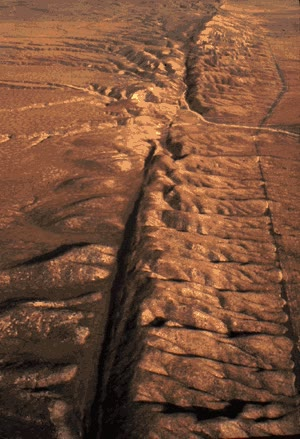
\includegraphics[width=0.28\linewidth]{images/book1/g7-usgs-san-andreas.jpg}

{\small कैलिफ़ोर्निया के कैरिज़ो \omterm{def:g1:landscapes-around-us:landform}{मैदान} को पार करता सैन एंड्रियास भ्रंश, हवाई
जहाज़ से: लंबी सीधी \omterm{def:g1:landscapes-around-us:landform}{घाटी} प्रशांत \omterm{def:g7:plate-tectonics:plate}{प्लेट} (बाएँ) और उत्तर अमेरिकी \omterm{def:g7:plate-tectonics:plate}{प्लेट} (दाएँ) के
बीच की सीमा है। फ़ोटो: रॉबर्ट वॉलेस, अमेरिकी भूवैज्ञानिक सर्वेक्षण (सार्वजनिक
डोमेन)।}
\end{omfigure}

\begin{method}[मानचित्र पर प्लेट सीमा पहचानना]\label{met:g7:plate-tectonics:recognise}
यह तय करने के लिए कि दो \omterm{def:g7:plate-tectonics:plate}{प्लेटों} को किस प्रकार की सीमा अलग करती है:
\begin{enumerate}
  \item \omterm{def:g7:plate-tectonics:plate}{प्लेटों} की गति के \omterm{def:g2:drawing-to-map:map}{मानचित्र} पर सीमा के दोनों ओर के तीर
        ढूँढो;
  \item अगर वे सीमा से दूर इशारा करते हैं, तो वह अपसारी है; अगर उसकी ओर, तो
        अभिसारी; अगर वे उसके समांतर हैं और विपरीत दिशाओं में इशारा करते हैं,
        तो रूपांतर;
  \item \omterm{def:g1:landscapes-around-us:landscape}{भूदृश्य} से जाँचो: किसी \omterm{def:g2:water-on-earth:ocean}{महासागर} के बीच में कटक या किसी \omterm{def:g3:continents-and-oceans:continent}{महाद्वीप} के
        आर-पार दरार \omterm{def:g1:landscapes-around-us:landform}{घाटी} \omterm{def:g7:plate-tectonics:plate-boundary}{अपसारी सीमा} के साथ होती है; \omterm{def:g4:volcanoes-earthquakes-first-look:volcano}{ज्वालामुखियों} की कतार वाली
        गहरी खाई, या एक ऊँची \omterm{def:g4:world-physical-map:range}{पर्वत-श्रेणी}, \omterm{def:g7:plate-tectonics:plate-boundary}{अभिसारी सीमा} के साथ; इनमें से कुछ भी
        नहीं, केवल एक लंबा सीधा भ्रंश, \omterm{def:g7:plate-tectonics:plate-boundary}{रूपांतर सीमा} के
        साथ।
\end{enumerate}
\end{method}

\section{प्लेटें कितनी तेज़ चलती हैं?}

\begin{proposition}[साल में कुछ सेंटीमीटर]\label{prop:g7:plate-tectonics:speed}
% ledger: data:pb2002 (speeds computed in figdata/grade-7/plate_speeds.py), usgs:mar-rate
दो पड़ोसी \omterm{def:g7:plate-tectonics:plate}{प्लेटें} एक-दूसरे के सापेक्ष साल में कुछ सेंटीमीटर की चाल से चलती
हैं: उत्तर अटलांटिक के आर-पार लगभग 2 सेंटीमीटर प्रति वर्ष से लेकर, पृथ्वी पर
सबसे तेज़ी से फैलने वाले कटक, पूर्वी प्रशांत उभार के आर-पार 14 सेंटीमीटर प्रति
वर्ष से ज़्यादा तक।
\end{proposition}

\begin{omfigure}
\begin{tikzpicture}
\begin{axis}[xbar, width=0.82\linewidth, height=5.4cm, xmin=0, xmax=16.5,
  ytick={1,...,6}, yticklabels={उत्तर अटलांटिक कटक, दक्षिण अटलांटिक कटक,
  सैन एंड्रियास भ्रंश, हिमालय, पेरू--चिली खाई, पूर्वी प्रशांत उभार},
  y tick label style={font=\small}, tick label style={font=\small},
  xlabel={एक प्लेट की दूसरी के सापेक्ष चाल (सेमी प्रति वर्ष)},
  label style={font=\small}, bar width=7pt, axis x line=bottom,
  axis y line=left, axis line style={-}, enlarge y limits=0.12,
  nodes near coords, nodes near coords style={font=\scriptsize},
  every node near coord/.append style={/pgf/number format/fixed,
  /pgf/number format/precision=1, /pgf/number format/fixed zerofill}]
\addplot[fill=omDef!55, draw=omDef!80!black] table[x=speed_cm_a, y=rank] {figdata/out/grade-7-plate_speeds.dat};
\end{axis}
\end{tikzpicture}

{\small छह सीमाओं पर \omterm{def:g7:plate-tectonics:plate}{प्लेटें} कितनी तेज़ चलती हैं: हर सीमा के साथ औसत, जो बर्ड
के \omterm{def:g7:plate-tectonics:plate}{प्लेट} मॉडल (2003) से निकाले गए हैं।}
\end{omfigure}

\begin{method}[सेंटीमीटर प्रति वर्ष से किलोमीटर प्रति मिलियन वर्ष तक]\label{met:g7:plate-tectonics:convert}
एक किलोमीटर \num{100000} सेंटीमीटर है। \qty{1}{cm} प्रति वर्ष की चाल अगर एक
मिलियन वर्ष तक बनी रहे, तो वह \num{1000000} सेंटीमीटर, यानी \qty{10}{km}, तय
करती है। इसलिए:
\[
  1\ \text{सेमी प्रति वर्ष} = 10\ \text{किमी प्रति मिलियन वर्ष}.
\]
सेंटीमीटर प्रति वर्ष वाली चाल को 10 से गुणा करो तो किलोमीटर प्रति मिलियन वर्ष
मिलते हैं; फिर मिलियन वर्षों की किसी संख्या से गुणा करो तो किलोमीटर में दूरी
मिलती है, या किसी दूरी को चाल से भाग दो तो समय मिलता है।
\end{method}

\begin{example}[अटलांटिक बढ़ता है]\label{ex:g7:plate-tectonics:atlantic}
% ledger: usgs:mar-rate
औसतन, मध्य-अटलांटिक कटक के दोनों किनारे लगभग \qty{2.5}{cm} प्रति वर्ष, यानी
\qty{25}{km} प्रति मिलियन वर्ष, की चाल से एक-दूसरे से दूर जाते हैं। 100
मिलियन वर्षों में इससे \qty{2500}{km} हो जाते हैं: काफ़ी समय तक बनी रहे, तो
एक जीवनकाल में पता न चलने जितनी धीमी चाल भी एक \omterm{def:g2:water-on-earth:ocean}{महासागर} खोल देती है।
\end{example}

\begin{remark}[आज गति को मापना]\label{rem:g7:plate-tectonics:gps}
% ledger: usgs:gps
ऐसी धीमी गतियाँ अब सीधे मापी जाती हैं। आधार-चट्टान में गड़े स्थायी स्टेशन
स्थिति बताने वाले उपग्रहों के संकेत पाते हैं और दिन-ब-दिन, कुछ मिलीमीटर तक,
अपनी स्थिति निकालते हैं। कुछ वर्षों में अलग-अलग \omterm{def:g7:plate-tectonics:plate}{प्लेटों} पर लगे स्टेशन
एक-दूसरे से दूर जाते या पास आते दिखते हैं, उन्हीं चालों से जो \omterm{def:g3:stones-pebbles-sand:rock}{चट्टानों} से
मिलियनों वर्षों के आधार पर निकाली गई हैं। उपग्रह से स्थिति निकालना अपने-आप में
\cref{ch:g9:maps-of-the-earth} का विषय है।
\end{remark}

\begin{omfigure}
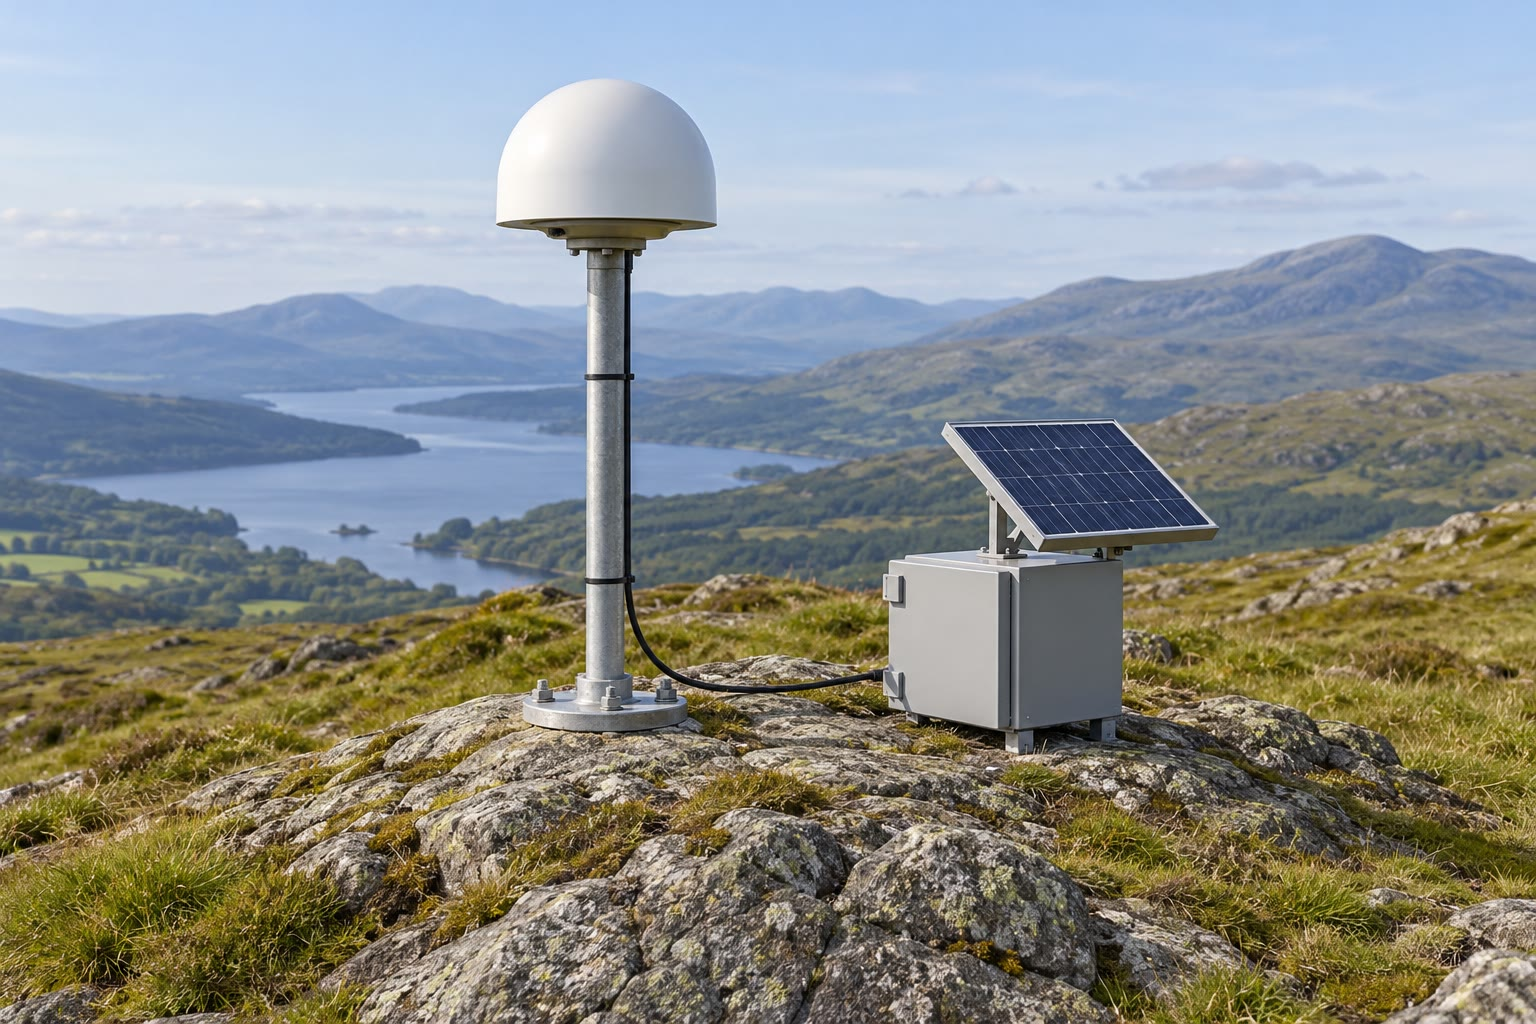
\includegraphics[width=0.55\linewidth]{images/book1/ai/g7-gps-station.jpg}

{\small स्थिति बताने वाला एक स्थायी स्टेशन: उसका एंटीना \omterm{def:g3:stones-pebbles-sand:rock}{चट्टान} में बोल्ट से
कसा है, इसलिए वह \omterm{def:g7:plate-tectonics:plate}{प्लेट} के साथ चलता है।}
\end{omfigure}

\section{अभ्यास}

\begin{exercise}[$\star$]\label{exo:g7:plate-tectonics:1}
\omterm{def:g7:plate-tectonics:continental-drift}{महाद्वीपीय विस्थापन} क्या है? उसका बचाव करने के लिए वेगनर ने जिन चार तरह के
सुरागों का उपयोग किया, उन्हें बताओ।
\end{exercise}

\begin{exercise}[$\star$]\label{exo:g7:plate-tectonics:2}
\omterm{def:g7:plate-tectonics:plate-boundary}{प्लेट सीमा} के तीन प्रकारों के नाम बताओ और हर एक के लिए बताओ कि दोनों \omterm{def:g7:plate-tectonics:plate}{प्लेटें}
एक-दूसरे के सापेक्ष कैसे चलती हैं।
\end{exercise}

\begin{exercise}[$\star$]\label{exo:g7:plate-tectonics:3}
\omterm{def:g4:volcanoes-earthquakes-first-look:earthquake}{भूकंपों} और \omterm{def:g4:volcanoes-earthquakes-first-look:volcano}{ज्वालामुखियों} का \omterm{def:g2:drawing-to-map:map}{मानचित्र} देखो। दुनिया के ऐसे दो क्षेत्रों के नाम
बताओ जहाँ बहुत-से बड़े \omterm{def:g4:volcanoes-earthquakes-first-look:earthquake}{भूकंप} आते हैं, और एक ऐसे \omterm{def:g3:continents-and-oceans:continent}{महाद्वीप} का जिसके बीच के
हिस्से में लगभग कोई \omterm{def:g4:volcanoes-earthquakes-first-look:earthquake}{भूकंप} नहीं आता।
\end{exercise}

\begin{exercise}[$\star$]\label{exo:g7:plate-tectonics:4}
\emph{मीसोसॉरस}, \omterm{def:g2:water-on-earth:salt-fresh}{मीठे पानी} में रहने वाले एक छोटे सरीसृप, के जीवाश्म ब्राज़ील
और दक्षिणी अफ़्रीका में मिलते हैं। यह इस बात का सुराग क्यों है कि दोनों
\omterm{def:g3:continents-and-oceans:continent}{महाद्वीप} कभी जुड़े थे?
\end{exercise}

\begin{exercise}[$\star\star$]\label{exo:g7:plate-tectonics:5}
अंटार्कटिका में कोयला मिलता है। इससे उस \omterm{def:g5:weather-and-climate:climate}{जलवायु} के बारे में क्या पता चलता है
जिसमें कोयला बना, और उस समय अंटार्कटिका कहाँ था, इसके बारे में हम क्या
निष्कर्ष निकाल सकते हैं?
\end{exercise}

\begin{exercise}[$\star\star$]\label{exo:g7:plate-tectonics:6}
बताओ कि इनमें से हर जगह पर किस प्रकार की सीमा है: मध्य-अटलांटिक कटक; एंडीज़;
सैन एंड्रियास भ्रंश; हिमालय; पूर्वी अफ़्रीकी दरार
\omterm{def:g1:landscapes-around-us:landform}{घाटी}।
\end{exercise}

\begin{exercise}[$\star\star$]\label{exo:g7:plate-tectonics:7}
\qty{2.5}{cm} प्रति वर्ष की चाल को किलोमीटर प्रति मिलियन वर्ष में बदलो। इस
चाल से, सीमा के दोनों ओर के दो बिंदु 60 मिलियन वर्षों में एक-दूसरे से कितनी
दूर हो जाएँगे?
\end{exercise}

\begin{exercise}[$\star\star$]\label{exo:g7:plate-tectonics:8}
1975 और 1984 के बीच --- नौ वर्षों में --- आइसलैंड में क्रैफ़्ला \omterm{def:g4:volcanoes-earthquakes-first-look:volcano}{ज्वालामुखी} के
पास की दरारें कुल मिलाकर लगभग \qty{7}{m} चौड़ी हो गईं। हर वर्ष औसतन कितने
सेंटीमीटर चौड़ाई बढ़ी? इसकी तुलना मध्य-अटलांटिक कटक की औसत चाल, लगभग
\qty{2.5}{cm} प्रति वर्ष, से करो, और सुझाओ कि ये दो संख्याएँ इतनी अलग क्यों
हैं।
\end{exercise}

\begin{exercise}[$\star\star$]\label{exo:g7:plate-tectonics:9}
वेगनर का सिद्धांत दशकों तक ठुकराया जाता रहा। वे किस प्रश्न का जवाब नहीं दे
सके? चलते \omterm{def:g3:continents-and-oceans:continent}{महाद्वीपों} की उनकी तस्वीर में \omterm{def:g7:plate-tectonics:plate-tectonics}{प्लेट विवर्तनिकी} का सिद्धांत क्या
बदलता है?
\end{exercise}

\begin{exercise}[$\star\star$]\label{exo:g7:plate-tectonics:10}
दो \omterm{def:g7:plate-tectonics:plate-boundary}{प्लेट सीमाओं} से होकर जाने वाली काट को देखो। \omterm{def:g2:water-on-earth:ocean}{समुद्र} की तली सबसे ऊँची कहाँ
है, और सबसे गहरी कहाँ? नई \omterm{def:g7:plate-tectonics:plate}{प्लेट} कहाँ बन रही है, और कोई \omterm{def:g7:plate-tectonics:plate}{प्लेट} वापस \omterm{def:g6:inside-the-earth:layers}{प्रावार} में
कहाँ जाती है?
\end{exercise}

\begin{exercise}[$\star\star\star$]\label{exo:g7:plate-tectonics:11}
पूर्वी प्रशांत उभार के आर-पार \omterm{def:g7:plate-tectonics:plate}{प्लेटें} लगभग \qty{14.2}{cm} प्रति वर्ष की चाल से,
और उत्तर अटलांटिक कटक के आर-पार लगभग \qty{2.2}{cm} प्रति वर्ष की चाल से
एक-दूसरे से दूर जाती हैं। पूर्वी प्रशांत उभार कितने गुना तेज़ है (निकटतम पूर्ण
संख्या तक)? हर कटक को \qty{1000}{km} नई समुद्री तली खोलने में कितना समय
लगता है?
\end{exercise}

\begin{exercise}[$\star\star\star$]\label{exo:g7:plate-tectonics:12}
% ledger: data:usgs-comcat, data:pb2002 (counts in figdata/grade-7/quakes_on_boundaries.py, part bands)
1976 से 2025 तक दर्ज परिमाण 6 या उससे ज़्यादा के 7\,031 \omterm{def:g4:volcanoes-earthquakes-first-look:earthquake}{भूकंपों} में से
4\,578 \omterm{def:g2:drawing-to-map:map}{मानचित्र} पर बनी \omterm{def:g7:plate-tectonics:plate-boundary}{प्लेट सीमा} की रेखा से \qty{100}{km} से कम दूरी पर आए,
6\,472 \qty{300}{km} से कम और 6\,786 \qty{500}{km} से कम दूरी
पर।
(क) रेखा से \qty{100}{km} और \qty{300}{km} के बीच कितने आए? (ख) निकटतम पूर्ण
संख्या तक निकालो: इन सभी \omterm{def:g4:volcanoes-earthquakes-first-look:earthquake}{भूकंपों} का कितना प्रतिशत रेखा से \qty{100}{km} से कम
दूरी पर आया? (ग) रेखा से \qty{100}{km} और \qty{300}{km} के बीच वाले बहुत-से
\omterm{def:g4:volcanoes-earthquakes-first-look:earthquake}{भूकंप} किसी गहरी महासागरीय खाई के एक ही ओर हैं। \omterm{def:g7:plate-tectonics:plate-boundary}{अभिसारी सीमा} पर जो होता है
उसका उपयोग करके समझाओ कि \omterm{def:g7:plate-tectonics:plate-boundary}{प्लेट सीमा} से पैदा होने वाला \omterm{def:g4:volcanoes-earthquakes-first-look:earthquake}{भूकंप} \omterm{def:g2:drawing-to-map:map}{मानचित्र} पर बनी
रेखा से इतनी दूर कैसे आ सकता
है।
\end{exercise}

\section{समस्या: दक्षिण अटलांटिक का खुलना}

\begin{problem}[{सप्ताहांत समस्या --- मानचित्र पर एक महासागर को मापना और यह
पता करना कि उसे खुलने में कितना समय लगा}]
\label{pb:g7:plate-tectonics:1}
% ledger: data:ne-land, earth:Rmean, data:pb2002, usgs:pangaea-breakup, usgs:atlantic-growth
% (all numbers computed in figdata/grade-7/south_atlantic.py: coasts at 23 S
% at 43.21 W and 14.39 E, 102.4 km per degree, AF-SA full rate 3.43 cm/yr)
दक्षिण अटलांटिक के एक \omterm{def:g2:drawing-to-map:map}{मानचित्र} पर एक विद्यार्थी \ang{23} दक्षिण \omterm{def:g6:latitude-longitude:latitude}{अक्षांश} वाली
\omterm{def:g6:latitude-longitude:latitude}{अक्षांश रेखा} पर उँगली चलाता है। यह रेखा रियो~डी~जनेरो के पास, \ang{43.2}
पश्चिम \omterm{def:g6:latitude-longitude:longitude}{देशांतर} पर, दक्षिण अमेरिका के \omterm{def:g1:landscapes-around-us:water}{तट} से निकलती है, \omterm{def:g2:water-on-earth:ocean}{महासागर} और
मध्य-अटलांटिक कटक को पार करती है, और वॉल्विस बे के पास, \ang{14.4} पूर्व
\omterm{def:g6:latitude-longitude:longitude}{देशांतर} पर, अफ़्रीका के \omterm{def:g1:landscapes-around-us:water}{तट} तक पहुँचती है। इस \omterm{def:g6:latitude-longitude:latitude}{अक्षांश रेखा} पर \omterm{def:g6:latitude-longitude:longitude}{देशांतर} का एक अंश
\qty{102}{km} का होता है। कटक के आर-पार, इस \omterm{def:g6:latitude-longitude:latitude}{अक्षांश} पर, दक्षिण अमेरिकी और
अफ़्रीकी \omterm{def:g7:plate-tectonics:plate}{प्लेटें} \qty{3.4}{cm} प्रति वर्ष की चाल से एक-दूसरे से दूर जाती हैं।

\begin{center}
\begin{tikzpicture}
\begin{axis}[axis equal image, xmin=-60, xmax=30, ymin=-42, ymax=12,
  width=0.6\linewidth, tick label style={font=\scriptsize},
  xtick={-60,-40,...,20}, ytick={-40,-20,0},
  xticklabel={$\pgfmathprintnumber{\tick}^\circ$},
  yticklabel={$\pgfmathprintnumber{\tick}^\circ$},
  axis background/.style={fill=omSea}]
\addplot[fill=omLithAlluv, draw=black!45, line width=0.3pt] table {figdata/out/shared-geo-land.dat};
\addplot[omRidge, line width=0.9pt, unbounded coords=jump, restrict x to domain=-45:5] table {figdata/out/shared-geo-school-ridge.dat};
\addplot[omRidge!70!black, line width=0.9pt, unbounded coords=jump, restrict x to domain=-45:5] table {figdata/out/shared-geo-school-transform.dat};
\draw[black, densely dashed, line width=0.7pt] (axis cs:-43.21,-23) -- (axis cs:14.39,-23);
\fill (axis cs:-43.21,-23) circle (1.5pt);
\fill (axis cs:14.39,-23) circle (1.5pt);
\node[font=\scriptsize, below right, inner sep=2pt] at (axis cs:-43.21,-23) {रियो~डी~जनेरो};
\node[font=\scriptsize, below left, inner sep=2pt] at (axis cs:14.39,-23) {वॉल्विस बे};
\node[font=\scriptsize, anchor=east, inner sep=1pt] at (axis cs:-16.5,-34) {मध्य-अटलांटिक कटक};
\end{axis}
\end{tikzpicture}
\end{center}

\medskip
\noindent\textbf{भाग I --- मेल के सुराग।}
\begin{enumerate}
  \item इस अध्याय के जीवाश्म \omterm{def:g2:drawing-to-map:map}{मानचित्र} पर उन जीवाश्मों के नाम बताओ जिनकी
        पट्टियाँ दक्षिण अमेरिका से अफ़्रीका में जाती हैं।
  \item \emph{मीसोसॉरस} के जीवाश्मों को एक ऐसे जानवर से क्यों नहीं समझाया जा
        सकता जो एक \omterm{def:g3:continents-and-oceans:continent}{महाद्वीप} से दूसरे तक तैरकर गया हो?
  \item दक्षिण अमेरिका का कौन-सा हिस्सा अफ़्रीका के किस हिस्से में बैठता है?
  \item आज दक्षिण अटलांटिक के बीचोंबीच किस प्रकार की \omterm{def:g7:plate-tectonics:plate-boundary}{प्लेट सीमा} चलती है? वहाँ
        दोनों \omterm{def:g7:plate-tectonics:plate}{प्लेटें} कैसे चलती हैं?
\end{enumerate}

\medskip
\noindent\textbf{भाग II --- महासागर को मापना।}
\begin{enumerate}[resume]
  \item \ang{23} दक्षिण वाली \omterm{def:g6:latitude-longitude:latitude}{अक्षांश रेखा} के साथ दोनों तटों के बीच \omterm{def:g6:latitude-longitude:longitude}{देशांतर} के
        कितने अंश हैं?
  \item इस \omterm{def:g6:latitude-longitude:latitude}{अक्षांश रेखा} के साथ \omterm{def:g2:water-on-earth:ocean}{महासागर} की चौड़ाई किलोमीटर में कितनी है? निकटतम
        दस किलोमीटर तक पूर्णांकित करो।
  \item \omterm{def:g3:continents-and-oceans:equator}{भूमध्य रेखा} पर \omterm{def:g6:latitude-longitude:longitude}{देशांतर} का एक अंश \qty{111}{km} का होता है। तो वह केवल
        \qty{102}{km} क्यों है, \ang{23} दक्षिण पर?
  \item कटक मोटे तौर पर \omterm{def:g2:water-on-earth:ocean}{महासागर} के बीचोंबीच चलता है। हर \omterm{def:g1:landscapes-around-us:water}{तट} कटक से लगभग कितनी
        दूर है?
\end{enumerate}

\medskip
\noindent\textbf{भाग III --- महासागर की उम्र।}
\begin{enumerate}[resume]
  \item जिस चाल से दोनों \omterm{def:g7:plate-tectonics:plate}{प्लेटें} एक-दूसरे से दूर जाती हैं, उसे किलोमीटर प्रति
        मिलियन वर्ष में बदलो।
  \item अगर \omterm{def:g2:water-on-earth:ocean}{महासागर} हमेशा इसी चाल से खुला होता, तो उसे अपनी आज की चौड़ाई तक
        पहुँचने में कितने मिलियन वर्ष लगते? निकटतम दस मिलियन वर्ष तक
        पूर्णांकित करो।
  \item भूवैज्ञानिक \omterm{def:g7:plate-tectonics:supercontinent}{पैंजिया} के टूटने का समय लगभग 225 से 200 मिलियन वर्ष पहले
        के बीच बताते हैं, और कहते हैं कि अटलांटिक पिछले 100 से 200 मिलियन
        वर्षों में बढ़ा है। क्या तुम्हारा जवाब इससे मेल खाता है?
  \item एक कारण बताओ कि दक्षिण अटलांटिक की असली उम्र तुम्हारी निकाली गई उम्र
        से अलग क्यों हो सकती है।
\end{enumerate}
\end{problem}
